%%    TEMPLATE for articles submitted to the full-tex econf proceedings
%%     
%%
%%     Please do not remove lines commented out with %+
%%           these are for the editors' use.
%%
%%     Questions?  Send email to :  mpeskin@slac.stanford.edu
%%   

\documentclass[12pt]{article}
\usepackage{epsfig}
% \usepackage[document]{ragged2e}
\usepackage{siunitx, dirtytalk, hyperref, nicefrac, mathtools} 
\usepackage{graphicx,sectsty,longtable,tocloft,color,pdfpages,sidecap,subfig,array,eurosym}
 \captionsetup[figure]{labelfont={bf},name={Fig.},labelsep=period}

\usepackage[english]{babel}
% smaller vertical spacing between references in bibliography
\let\OLDthebibliography\thebibliography
\renewcommand\thebibliography[1]{
  \OLDthebibliography{#1}
  \setlength{\parskip}{0pt}
  \setlength{\itemsep}{0pt plus 0.3ex}
}

\usepackage{lmodern} % for bold teletype font
\usepackage{listings}
\usepackage{color}
\definecolor{codegreen}{rgb}{0,0.6,0}
\definecolor{codegray}{rgb}{0.5,0.5,0.5}
\definecolor{codepurple}{rgb}{0.58,0,0.82}
\definecolor{backcolour}{rgb}{0.95,0.95,0.92}
\lstdefinestyle{mystyle}{
    backgroundcolor=\color{backcolour},   
    commentstyle=\color{codegreen},
    keywordstyle=\color{magenta},
    numberstyle=\tiny\color{codegray},
    stringstyle=\color{codepurple},
    basicstyle=\footnotesize,
    breakatwhitespace=false,         
    breaklines=true,                 
    captionpos=b,                    
    keepspaces=true,                 
    numbers=left,                    
    numbersep=5pt,                  
    showspaces=false,                
    showstringspaces=false,
    showtabs=false,                  
    tabsize=2
}
\lstset{style=mystyle}

%%%%%%%%%%%%%%%%%%%%%%%%%%%%%%%%%%%%%%%%%%%%%%%%%%%%%%%%%%%%%%%%%%%%%%%%%%%%
%%  Do not change these:
\textwidth=6.0in  \textheight=8.25in

%%  Adjust these for your printer:
\leftmargin=-0.3in   \topmargin=-0.20in


%%%%%%%%%%%%%%%%%%%%%%%%%%%%%%%%%%%%%%%%%%%%%%%%%%%%%%%%%%%%%%%%%%%%%%%%%%%%
%  personal abbreviations and macros
%    the following package contains macros used in this document:
% \input LinksAndMetadata.tex
%%%%%%%%%%%%%%%%%%%%%%%%%%%%%%%%%%%%%%%%%%%%%%%%%%%%%%%%%%%%%%%%%%%%%%%%%%%
%
%  To include an item in the INDEX of the conference volume,
%           flag it with    \index{<item name>}
%  The use of this macro is illustrated in the text.
%
%%%%%%%%%%%%%%%%%%%%%%%%%%%%%%%%%%%%%%%%%%%%%%%%%%%%%%%%%%%%%%%%%%%%%%%%%%%%%

\def\Title#1{\begin{center} {\Large {\bf #1} } \end{center}}

\begin{document}


\Title{Manual: Internal tracker alignment for the $g-2$ experiment}

\bigskip\bigskip

%+\addtocontents{toc}{{\it D. Reggiano}}
%+\label{ReggianoStart}

\begin{raggedright}  
Gleb Lukicov$\,^{a,}$\footnote{g.lukicov@ucl.ac.uk}\\
{\it $^{\mathrm{a}}$Department of Physics and Astronomy, University College London, London, \\ WC1E 6BT, United Kingdom}
\bigskip\bigskip
\end{raggedright}

\begin{center}
\today
\end{center}

\null\vspace{\fill}
\begin{abstract}
This document outlines the need for the internal alignment of the tracking detectors, and the methodology of the alignment. The software methods used in the alignment are summarised to allow for the future alignment constants to be established for Run-3 and beyond. Internal alignment of the trackers in Run-1 and Run-2 has been established, with the constants defined as the interval of validity (IoV) in the reconstruction database. 
\end{abstract}
\vspace{\fill}

\tableofcontents

\clearpage

\section{Introduction}
In order for the tracking detector to reduce the systematic uncertainty on the $a_{\mu}$ measurement and improve the sensitivity to a muon EDM, a precise calibration of the tracking detector is required. One of such calibrations is the internal alignment, which considers the positions of the tracking modules within a station. 

Track-based internal alignment of the two stations of the tracking detector was implemented using data from Run-1 and Run-2. A Monte Carlo simulation was also developed to understand the detector geometry, and how the detector geometry affects how well the alignment can be determined, as well as to test the alignment procedure itself. A single figure-of-merit emphasising the need for a well aligned detector is shown in Fig.~\ref{fig:rad_inter}, which highlights that even a relatively small scale of misalignment can have a large impact on the detector performance w.r.t to the beam extrapolation. Additionally, alignment is essential for setting a new limit on the muon EDM. Broadly speaking, an internal misalignment of an element of a tracking detector manifests as a presence of a large residual between a measurement (e.g. DCA of a hit to a wire) and a DCA of a fitted track to that wire. This large residual arises from the fact that the assumed detector position, which was used in the fitting of the track, is not the actual position of that detector. The aim of the alignment procedure is to establish the corrections to the assumed detector position, and hence, minimise the residuals.

\begin{figure}[h!]
\centering
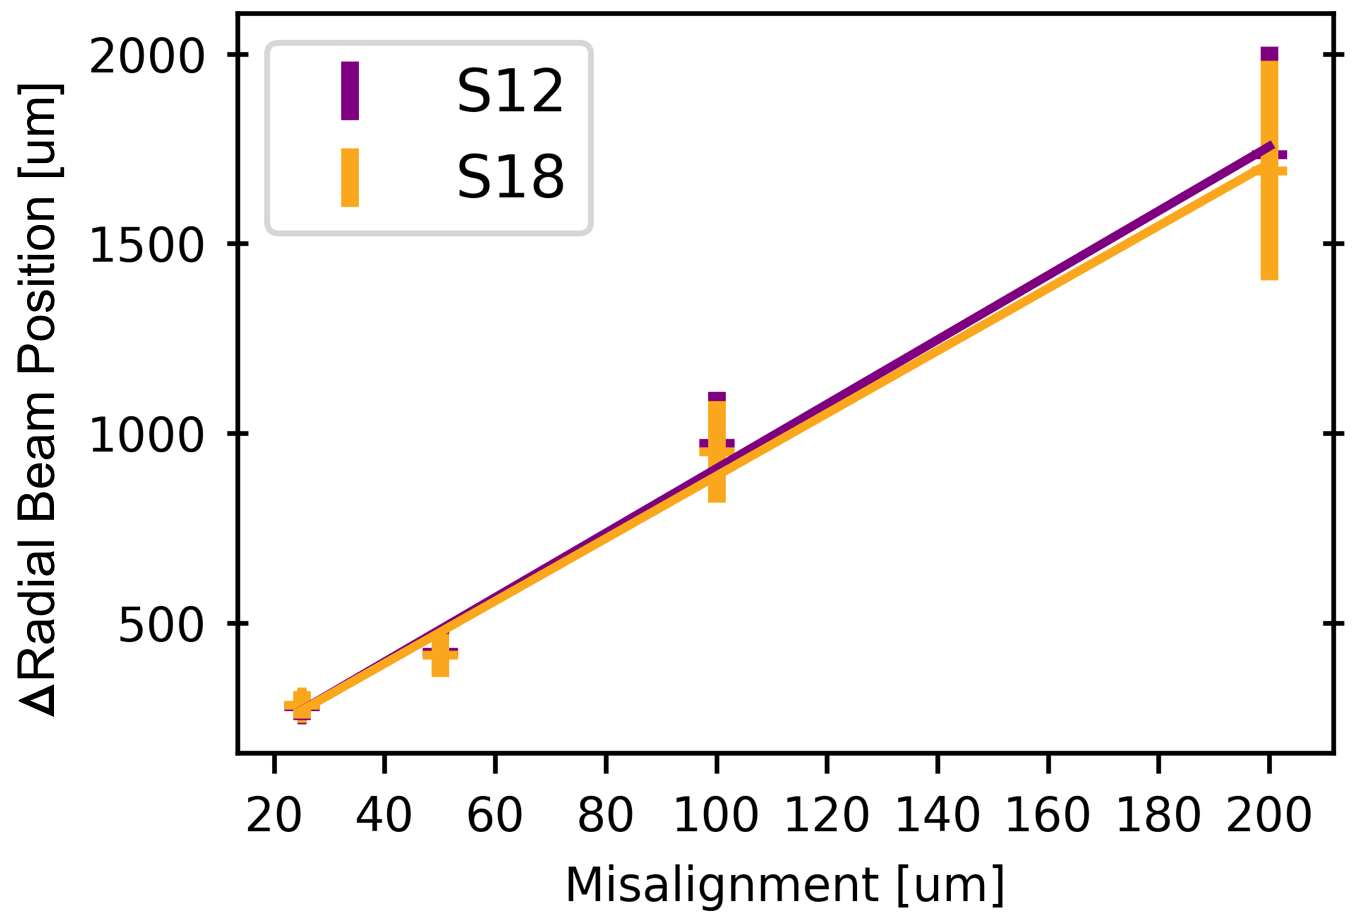
\includegraphics[width=0.6\linewidth]{fig/internal_rad.png}
\caption{Detector response to a uniform radial misalignment at different scales w.r.t to the difference in the extrapolated radial position.}
\label{fig:rad_inter}
\end{figure}

\section{Methodology of the alignment of the trackers}
The chosen alignment framework was \texttt{Millepede-II} \cite{mp2}, which utilises a simultaneous fit of many parameters describing the detector geometry and the input data. Under this method correlations between different alignment parameters are taken into account, to produce an unbiased corrections to the position of the detector. The definition of the coordinate system used is shown in Fig~\ref{fig:Rotation}.

\begin{figure}[h!]
\centering
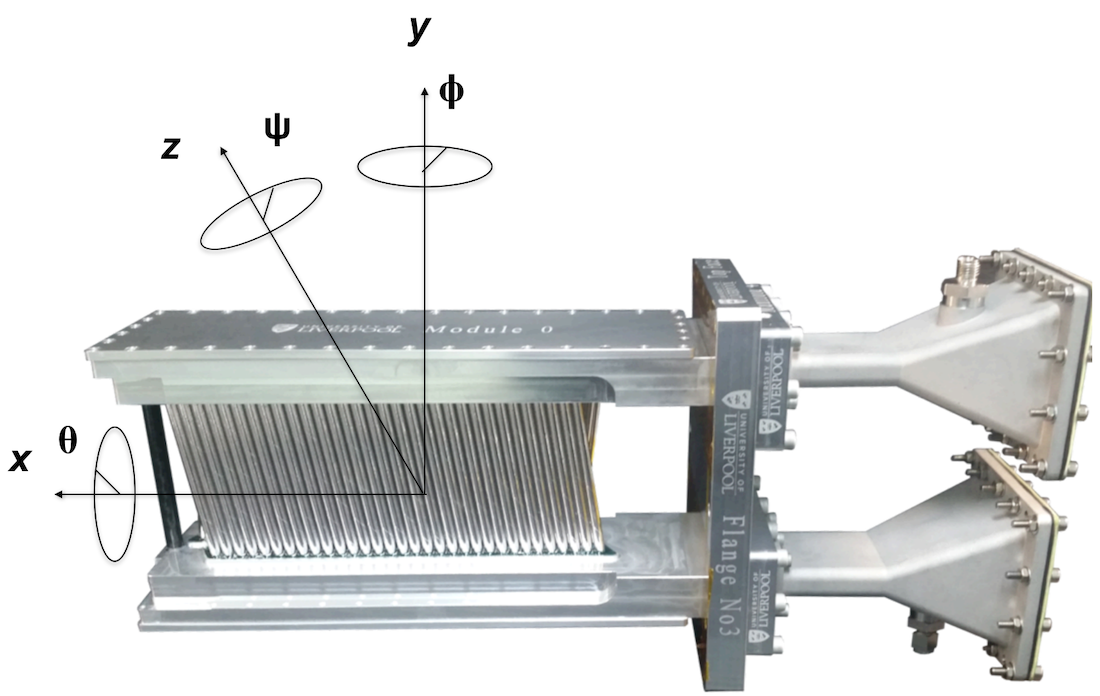
\includegraphics[width=0.6\linewidth]{fig/rotAxis.png}
\caption{Convention for misalignments (translations and rotation) in a module coordinate system. The positive radial and vertical shifts are along $x$ and $y$, respectively.}
\label{fig:Rotation}
\end{figure}

The alignment task can be summarised as a Least Squares Fit (LSF) problem with a very large number of parameters. These parameters can be divided into two classes: global and local parameters. Global parameters (i.e. the alignment parameters) affect all tracks (e.g. radial position of a detector). Local parameters are associated with individual fitted tracks. For example, a straight line fit in 2D will have 2 local parameters: a slope and an intercept. \texttt{Millepede-II} solves the linear LSF problem with a simultaneous fit of all global and local parameters minimising a linearised function of a sum of residuals. An objective function, $F$, is then minimised with respect to a variation of global and local parameters
\begin{equation}
\label{eq:obj_fun}
F(\boldsymbol{a},\boldsymbol{b})=\frac{\partial\chi^2(\boldsymbol{a},\boldsymbol{b})}{\partial(\boldsymbol{a},\boldsymbol{b})}=
\sum_{j}^{tracks}\sum_{i}^{hits} \frac{1}{(\sigma^{\mathrm{det}}_{i,j})^2} \frac{\big(r_{i,j}(\boldsymbol{a_0},\boldsymbol{b_0}_{,j})+\frac{\partial r_{i,j}}{\partial \boldsymbol{a}}
\delta \boldsymbol{a} +\frac{\partial r_{i,j}}{\partial \boldsymbol{b}_j}\delta \boldsymbol{b}_j\big)^2}{\partial(\boldsymbol{a},\boldsymbol{b})}=0,
\end{equation}
where $\boldsymbol{a_0}$ and $\boldsymbol{b_0}$ are the initially assumed geometry and track parameters, respectively, $r$ is the track residual (as shown in Fig.~\ref{fig:DriftCylinder}), and $\sigma^{\mathrm{det}}$ is the detector resolution. The corrections to the global parameters, $\delta\boldsymbol{a}$, allow for the minimisation of $F$, and are results of the alignment procedure. These corrections are then added to the assumed geometry of the detector to improve its performance.

\begin{figure}[tbp]
\centering
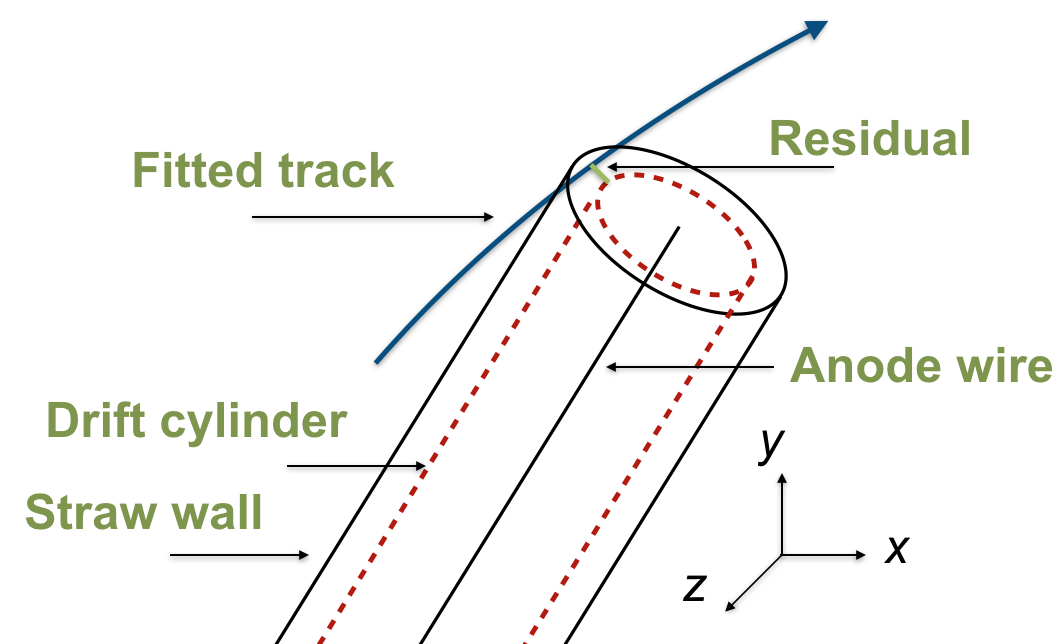
\includegraphics[scale = 0.45]{fig/DriftCylinder.png}  
    \caption{Visualisation of the drift cylinder, which is defined by the measured drift time in the straw.}
\label{fig:DriftCylinder} 
\end{figure}

\section{Alignment results and references}
In simulation (MDC1), alignment stability was reached, and alignment convergence within \SI{2}{\micro\metre} and \SI{10}{\micro\metre} radially and vertically, respectively, was established as shown in \textbf{\href{https://gm2-docdb.fnal.gov/cgi-bin/private/ShowDocument?docid=17551}{DocDB:17551}}. Stable alignment results and improved residuals in data, using run 15922, were reached as shown in \textbf{\href{https://gm2-docdb.fnal.gov/cgi-bin/private/ShowDocument?docid=17722}{DocDB:17722}}.

Stability of the alignment constants across 3 intervals of validity (IoV) of Run-1 and Run-2 are shown in \textbf{\href{https://gm2-docdb.fnal.gov/cgi-bin/private/ShowDocument?docid=19294}{DocDB:19294}}.

A more detailed description of the alignment methods is contained in \textbf{\href{https://gm2-docdb.fnal.gov/cgi-bin/private/ShowDocument?docid=15106}{DocDB:15106}} (\textbf{see backup also}). More details can also be found in \textbf{\href{https://gm2-docdb.fnal.gov/cgi-bin/private/ShowDocument?docid=9245}{DocDB:9245} (toy model in 2D)}, \textbf{\href{https://gm2-docdb.fnal.gov/cgi-bin/private/ShowDocument?docid=11331}{DocDB:11331} (residual derivatives)}, \textbf{\href{https://gm2-docdb.fnal.gov/cgi-bin/private/ShowDocument?docid=15382}{DocDB:15382} (progress in MDC1)}. 

The uncertainty on the beam extrapolation due to the misalignment was estimated in \textbf{\href{https://gm2-docdb.fnal.gov/cgi-bin/private/ShowDocument?docid=16685}{DocDB:16685}}. 

A key point to note from the documents listed above is that the alignment is an iterative process. A preliminary alignment constants (i.e. module positions) from iteration 1 are used for re-tracking, with alignment at iteration 2 and beyond taking improved tracks as in input for the LSF. Three iterations are usually enough to reach convergence, which is seen as $\delta\boldsymbol{a} \rightarrow 0$. The iterations mentioned here are external to the \texttt{Millepede-II} framework, which has its own internal iterations for matrix inversion and LSF; description of \texttt{Millepede-II} is beyond the scope of this document, and is contained in the official manual \cite{mp2}.   

\section{Software methods}
The alignment software is part of the \verb!gm2tracker! project: \verb!gm2tracker/align/!. An alignment software module has been developed as part of the \textit{gm2 art} software framework. This module comes last in the tracking chain, taking the final track-data product (\verb!TrackArtRecords_tracks!) from either data or simulation. The description of the tracking software\footnote{Geane track fitting was developed by Nick} and data products is contained in a separate manual \cite{Nick}. The geometry is fully described at the tracking stage and is passed to the alignment module in the \verb!beginRun()! function. The alignment module (\verb!TrackerAlignment!) calculates the residuals of the selected tracks, as well as computes the local and global derivatives \textbf{(see backup of \href{https://gm2-docdb.fnal.gov/cgi-bin/private/ShowDocument?docid=11331}{DocDB:11331})}. A \verb!C++! infrastructure (\texttt{Mille}) is provided \cite{mp2} to write this information into a binary file (\textbf{alignment data}) which is passed to \texttt{PEDE} (a \texttt{Fortran} executable), which performs a simultaneous LSF via a matrix inversion. The alignment module is also responsible for writing a constraints file (specifying the redundant degrees of freedom), and a steering file (specifying the mathematical methods used by \texttt{PEDE}). The final outputs of the \texttt{PEDE} algorithm are labels and the corresponding fitted values of the global parameters (module positions) and their errors, if applicable. This algorithm is shown in Fig.~\ref{fig:mp2}.\\
\vspace{-0.5cm}
\begin{figure}[h!]
    \centering
    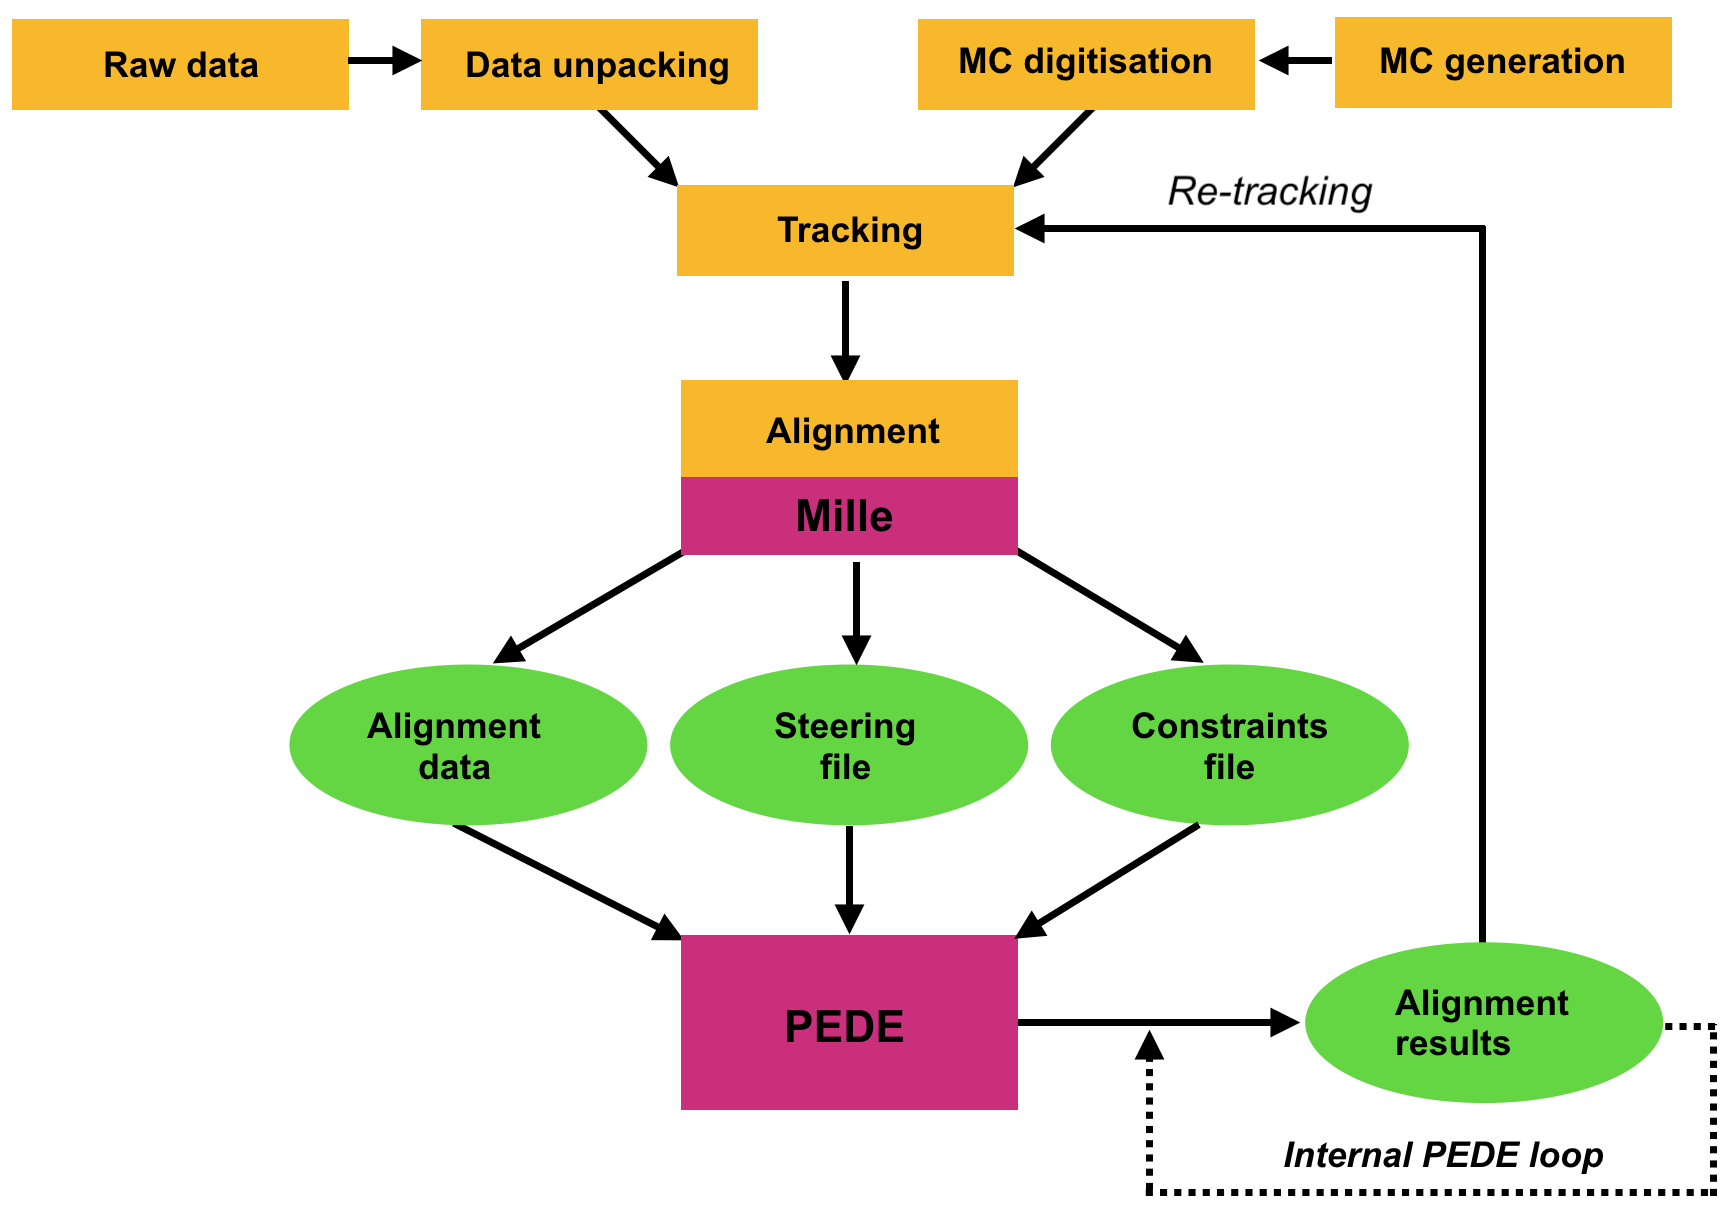
\includegraphics[scale = 0.40]{fig/MP2.png}
    \caption{The schematic of the \texttt{Millepede-II} routine (shown in purple) with the \textit{gm2 art} software framework (shown in orange). The final result of alignment is then used in tracking to improve the residuals.}
    \label{fig:mp2}
\end{figure}
\clearpage
\subsection{Alignment module: TrackerAlignment} \label{sub:alignment_module}
The \textit{producer} alignment module is controlled by a FHICL file, for example for S12, \\\verb!trackerAlignment_S12.fcl!. The FHICL file controls the applied cuts on the tracks that will be used for alignment, and specifies the methods that will be used by \texttt{PEDE}.

A \textit{dubug} mode is available when not monitoring the alignment over large datasets, with \verb!monitoring : false!. This way, a \verb!ROOT! file with debug plots will be produced. One must also set: \\
\lstinline{outputCommands : [``drop *'', ``keep gm2strawtracker::TrackerAlignmentArtRecords_*_*_*'']} \\
in the FHICL file, as well as add \lstinline{plotsPath : [ outputArtRootFile ]}, to produce the \verb!gm2tracker_reco.root! file, from which analysis-level alignment plots \\ (\verb!TrackerAlignment.root!) can be produced with \verb!RunAlignmentPlots.fcl!. \\The data product for the alignment is described in \\ \verb!gm2dataproducts/strawtracker/TrackerAlignmentArtRecord.hh!.   

\subsection{Tracking cuts for alignment}
The following cuts were used to select tracks, from simulation or data, to be used in the alignment framework:
\begin{itemize}\setlength\itemsep{0.05em}\small
    \item \textbf{Maximum layers with multiple hits = 0.} Only select tracks that have unambiguous set of hits in a single straw per layer. 
    \item \textbf{DCA \textgreater~\SI{500}{\micro\metre}.} A hit with a small DCA is not used in the alignment. This is required due to the derived residual continuity as we cross the L/R boundary.
    \item \textbf{pValue \textgreater~ 0.005.} Only tracks that has a reasonable fit quality are used. 
    \item \textbf{Hits \textgreater~ 9.} Only using tracks that have hits in at least three modules. 
    \item \textbf{\nicefrac{Pz}{P} \textgreater~ 0.93.} Tracks that have large curvature are removed.
\end{itemize}

\subsection{Installing and controlling \texttt{PEDE}} 
The \texttt{PEDE}, which a \texttt{Fortran} executable, is not part of art. The produced binary data can be passed to a standalone \texttt{PEDE} installation on \texttt{gm2gpvm}. The instruction to install \texttt{PEDE} are located on the \textbf{\href{https://cdcvs.fnal.gov/redmine/projects/gm2tracker/wiki/Tracker_Alignment_MC_with_Millipede_II_Framework}{gm2tracker Redmine WIKI}}. 
The \texttt{PEDE} is controlled via a steering file, which, as well as the constraints file, are produced automatically via the \verb!TrackerAlignment! module:
\lstinputlisting[language=Bash]{Steer.sh}
\clearpage

The constraint equation is given by
\begin{equation}
        c = \sum_i^N l_i\cdot f_l,
\end{equation}
where $c$ is is the constraint value, $l$ is the global parameter label, $f$ is the parameter factor\footnote{See \texttt{Millepede-II} manual \cite{mp2}}, and the summation is taken over the parameters contributing to the constraint. In the particular case of the alignment of the tracking detector radially and vertically with curved tracks in a magnetic field, five global degrees of freedom must be fixed by the constraints. There are two overall translations, radially and vertically, that must sum to 0, as well as two global angles of rotations, which are also fixed at 0. The global rotation is defined through the centre of the station. This is done to minimise the \say{lever arm effect}. The fifth constraint deals with the radial \textit{bowing effect} due to the radially curving tracks in the magnetic field. The constraint equations can be formulated as follows, for example for station 12:
\begin{enumerate}
    \item No overall radial translation
    \begin{equation}
        0.0 = \sum_{i=1}^N l_i\cdot 1 = 1211 \cdot 1 + 1221 \cdot 1 + ... 1281 \cdot 1,
    \end{equation}
    where, for example, label $1281$ corresponds to station number 12, module number 8 and parameter number 1 (i.e. radial shift). The factor of $1$ simply means equal weighting for all parameters. The above equation is written in the PEDE format as follows
    \lstinputlisting[language=Bash]{RadCont.sh}
    \item No overall vertical rotation
    \begin{equation}
        0.0 = \sum_{i=1}^N l_i\cdot (N+1-2\cdot i)  = 1212 \cdot 7 + 1222 \cdot 5 + ... 1282 \cdot -7,
    \end{equation}
    \lstinputlisting[language=Bash]{RotCont.sh}
    \item Constraint the radial bowing effect
     \begin{equation}
        0.0 = \sum_i^N l_i\cdot (N+1-2\cdot i)^2 = 1211 \cdot 49 + 1221 \cdot 25 + ... 1281 \cdot 49, \label{eq:bowing}
    \end{equation}
    \lstinputlisting[language=Bash]{CurveCont.sh}
\end{enumerate}
The constrains can be summarised as follows, the radial constraints equation
\begin{equation}
    0=a(x-x_0)^2+b(x-x_0)+c,   
\end{equation}
and the vertical constraints equation  
\begin{equation}
    0=b(x-x_0)+c,
\end{equation}
where $x_0=\SI{482.394}{\milli\metre}$ is the centre of the station.

The motivation behind constraining the overall translations and rotations is simple: internal alignment should not return the module offsets related to the global movements. These global movements have been independently measured\footnote{Global alignment was established by Joe, Leah, and Horst.} by the global alignment \cite{Joe}. The constraint on the radial bowing effect deserves a special mention, as it is essentially a \say{local minima problem}: the internal alignment can place the tracker modules along a curved path, as the residuals will be unchanged. This radial detector curvature, however, will change the measurement of the momentum of the tracks, and the extrapolated radial position. The detector curvature, therefore, must be measured and eliminated by another means, as described in \textbf{\href{https://gm2-docdb.fnal.gov/cgi-bin/private/ShowDocument?docid=18625}{DocDB:18625}}.


\subsection{Ancillary scripts}
There is a lot of developed infrastructure to simplify the alignment routines in \\ \verb!gm2tracker/align/macros/!. Some of the essential scripts are summarised here: 
\begin{itemize}\setlength\itemsep{0.05em}\small
    \item \verb!GetRes.py!: Produces residual plots\footnote{S12 and S18 must be specified for GeanePlots, as in the align/fcl/RunTrackingPlots\_align.fcl} on \verb!trackRecoPlots.root! or \verb!TrackerAlignment.root!
    \item \verb!GetRes_Iter.py!: Produces residual comparison plots before and after alignment from two \verb!TrackerAlignment.root! files
    \item \verb!RobustTrackerLaunch.py!: Produces a visual representation of the modules offsets and produces \verb!OffsetsPerModule.fcl! file that can be used for re-tracking  
    \item \verb!Rename.sh!: Renames \verb!.root! files into \verb!.bin! on the returned alignment data files form the grid. See \textbf{\href{https://redmine.fnal.gov/redmine/projects/g-2/wiki/Job_Running_Submission_FAQ\#What-if-I-would-like-to-retrieve-output-files-with-different-extension-like-a-binary-file-bin-produced-by-my-jobs}{Grid Wiki: "What if I would like to retrieve output file(s) with different extension? like a binary file (.bin) produced by my jobs?"}} and \textbf{\href{https://gm2-docdb.fnal.gov/cgi-bin/private/ShowDocument?docid=18826}{DocDB:18826}} 
    \item \verb!PEDEParallel.py!: Produces multiple steering files and runs \texttt{PEDE} in parallel on many runs 
       \item \verb!monitor.py!: Produces the final monitoring plot across many runs 
\end{itemize}
\subsection{Run alignment locally}
One can start with raw \texttt{MIDAS} data, unpack it (\verb!runStrawUnpacker.fcl!), and reconstruct tracks (\verb!RunTrackingDAQ.fcl!), as described in \textbf{\href{https://gm2-docdb.fnal.gov/cgi-bin/private/ShowDocument?docid=19297}{DocDB:19297}}. The alignment can then be run locally on the tracks (e.g. \verb!run15922_tracks.root!)
\begin{lstlisting}[language=bash] 
     gm2 -c trackerAlignment_S18.fcl -s myDataSet_subrun.root \end{lstlisting}
This will produce \verb!SteeringFile.txt!, \verb!ConstraintFile.txt! and binary data file \verb!Data.bin!. To get the alignment correction for these tracks, \verb!PEDE! is run with
\begin{lstlisting}[language=bash] 
     PEDE SteeringFile.txt \end{lstlisting}
If debug mode was selected, as described in Sc.\ref{sub:alignment_module}, analysis-level plots can be produced to check the residuals and derivatives via
\begin{lstlisting}[language=bash] 
    gm2 -c RunAlignmentPlots.fcl -s gm2tracker_reco.root\end{lstlisting}

\subsection{Run iterative alignment on a single run with residual verification}\label{sub:run_iterative}
Refer to the \textbf{\href{https://redmine.fnal.gov/redmine/projects/g-2/wiki/Job_Running_Submission_FAQ}{Grid Wiki}} on how to \textit{create} and \textit{pre-stage} a SAM dataset. 

One can start with raw \texttt{MIDAS} data, unpack it (\verb!runStrawUnpacker.fcl!), and reconstruct tracks (\verb!RunTrackingDAQ.fcl!), as described in \textbf{\href{https://gm2-docdb.fnal.gov/cgi-bin/private/ShowDocument?docid=19294}{DocDB:19294}}. Assuming this has been done, or a dataset (e.g. \texttt{myDataSet}) containing tracks from, for example, 450 subruns from a single run exists, alignment is done as follows.

\begin{enumerate}
    \item Submit an alignment grid job (with the default FHICL parameters) for S18:
    \begin{lstlisting}[language=bash]
     ./gridSetupAndSubmitGM2Data.sh --daq --reco --fcl=gm2tracker/align/fcl/trackerAlignment_S18.fcl --localArea --output-dir=/pnfs/GM2/scratch/users/AAA/S18_align --sam-dataset=myDataSet --multipleroot --njobs=450 \end{lstlisting}
     \item Rename files in \verb!S18_align/DATE/data! to \verb!.bin!
     \begin{lstlisting}[language=bash] 
     Rename.sh /pnfs/GM2/scratch/users/AAA/S18_align/DATE/data/\end{lstlisting}
     \item As \verb!.txt! files are not returned by the grid (one can never have it all!) a local alignment jobs must be run to have the steering and constraint files
     \begin{lstlisting}[language=bash] 
     gm2 -c trackerAlignment_S18.fcl -s myDataSet_subrun.root \end{lstlisting}
     \item Add full paths of the renamed \verb!.bin! files from \verb!S18_align/DATE/data! to the SteeringFile.txt
     \item Run \texttt{PEDE}
     \begin{lstlisting}[language=bash] 
     PEDE SteeringFile.txt \end{lstlisting}
     \item Produce offsets (\verb!OffsetsPerModuleS18.fcl!) and their plots (from the results file \verb!millipede.res!), as shown in Fig.~\ref{fig:Align_Data}. If used as part of an iteration, another option (e.g. for iteration 2) \lstinline{--offset_file=RunTrackerDAQ_Iteration2.fcl} must be used to supply the previous set of alignment results for comparison.
     \begin{lstlisting}[language=bash] 
     python RobustTrackerLaunch.py --pede_file=millipede.res \end{lstlisting}
     \begin{figure}[ht!]
        \centering
        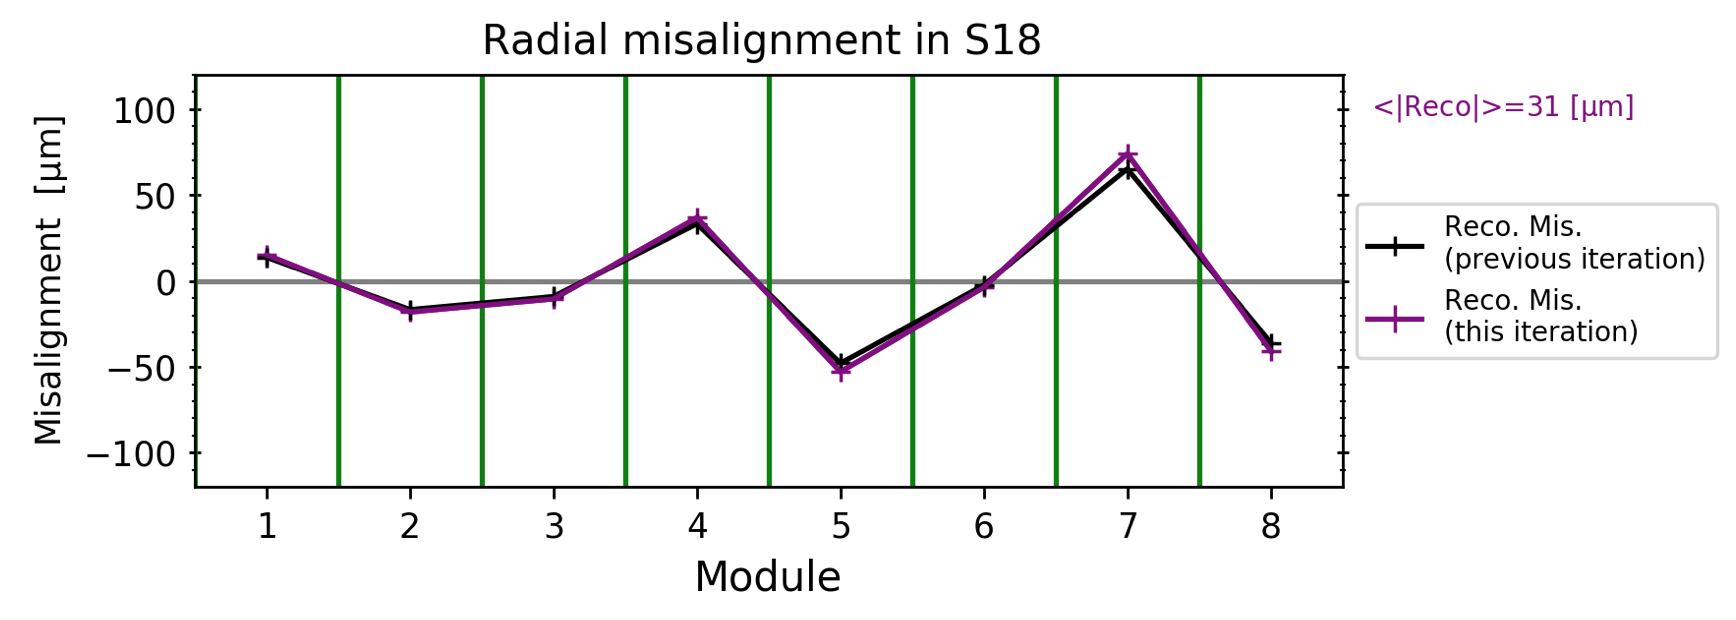
\includegraphics[width = 0.7\linewidth]{fig/Align_Data.png}
        \caption{The alignment results with $10^5$ tracks after 2 iterations. The alignment stability is not yet reached, as seen by the alignment results from the previous iteration (shown in black) and current iteration (purple) not converged.}
        \label{fig:Align_Data}
    \end{figure}
     \item Add the resultant \verb!OffsetsPerModuleS18.fcl! to end of the \\ \verb!RunTrackingDAQ_Iteration2.fcl! and re-track on the grid, defining a new dataset \texttt{myDataSetIteration2}
     \item Repeat steps $1-7$, until the results from the current iteration are same as the last one
      \item Produce the final residual comparison plots, for example, for the first and third iteration as shown in Fig.~\ref{fig:Res_Data}. \textbf{S12 and S18 must be specified for separate instances of GeanePlots, as shown in \small{\texttt{align/fcl/RunTrackingPlots\_align.fcl}}, to produce residuals separately for each station}. Alternatively, run directly on \verb!TrackerAlignment.root!
     \begin{lstlisting}[language=bash] 
     GetRes_Iter.py --fileN1=Iter1/TrackerAlignment.root --fileN1=Iter3/TrackerAlignment.root \end{lstlisting}
     \end{enumerate}
     \vspace{-0.5cm}
     \begin{figure}[ht]
    \centering
    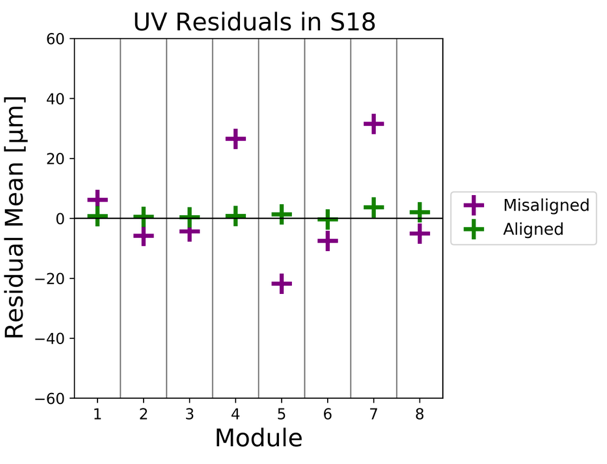
\includegraphics[width = 0.5\linewidth]{fig/Res_Data.png}
    \vspace{-0.2cm}
    \caption{An improvement in the residual means after the alignment (3 iterations) is clear.}
    \label{fig:Res_Data}
    \end{figure}

\subsection{Run alignment monitoring}
The goal here is to check that across an entire dataset or a whole Run (e.g. Run-1), the alignment is stable. For example, for an entire \textit{60-hour} dataset with the dataset name \verb!gm2pro_daq_full_run1_60h_5037A_goldList!:
\begin{enumerate}
    \item Submit an alignment grid job (with the default FHICL parameters) for S12:
    \begin{lstlisting}[language=bash]
     ./gridSetupAndSubmitGM2Data.sh --daq --reco --fhiclFile=trackerAlignment_S12.fcl --localArea --output-dir=/pnfs/GM2/scratch/users/AAA/gm2pro_daq_full_run1_60h_5037A_goldList/S12/ --sam-dataset=gm2pro_daq_full_run1_60h_5037A_goldList --noifdh_art --onebyone --multipleroot --njobs 5000 \end{lstlisting}
     \item Rename files in \verb!S18_align/DATE/data! to \verb!.bin!
     \begin{lstlisting}[language=bash] 
     Rename.sh /pnfs/GM2/scratch/users/AAA/S18_align/DATE/data/\end{lstlisting}
     \item Run script that will take care of preparing steering and constraint files for each run in the new folder \verb!Monitoring! (use full paths e.g. \verb!/pnfs/GM2/....!)
        \begin{lstlisting}[language=bash]
      python gm2tracker/align/macros/PEDEParallel.py --mode=prepare --inputData=gm2pro_daq_full_run1_60h_5037A_goldList/S12/DATE/data/ \end{lstlisting}
      \item Run the same script in \verb!pede! and then \verb!align! modes to first run \verb!PEDE! and then \verb!RobustTrackerLaunch.py! on each run
        \begin{lstlisting}[language=bash]
      python gm2tracker/align/macros/PEDEParallel.py --mode=pede --inputData=gm2pro_daq_full_run1_60h_5037A_goldList/S12/DATE/data/Monitoring/ 
      python gm2tracker/align/macros/PEDEParallel.py --mode=align --inputData=gm2pro_daq_full_run1_60h_5037A_goldList/S12/DATE/data/Monitoring/\end{lstlisting}
       \item Finally, produce a monitoring plot as shown in Fig.~\ref{fig:60h}.
      \begin{lstlisting}[language=bash]
      python $MP2/monitor.py -s12 S12/ -s18 S18 \end{lstlisting}
    \end{enumerate}
    \vspace{-0.5cm}
    \begin{figure}[!ht]
    \centering
    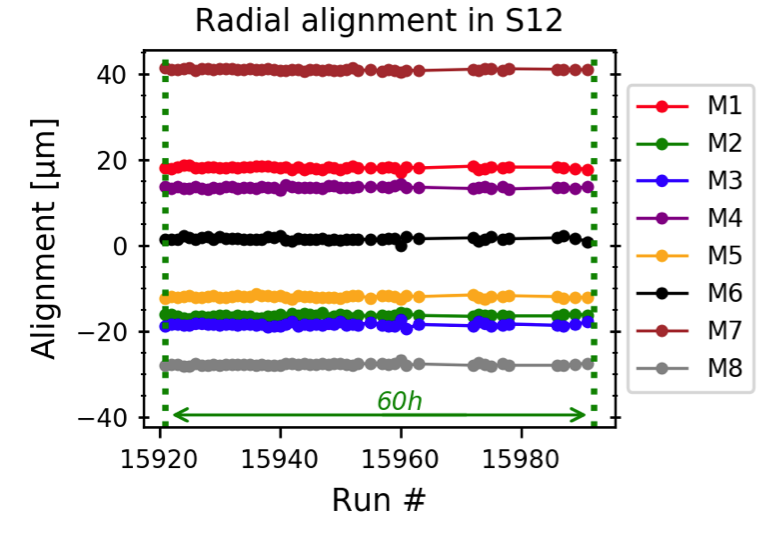
\includegraphics[width = 0.5\linewidth]{fig/60h.png}
    \vspace{-0.2cm}
    \caption{Radial alignment results in the eight modules of station 12 across 60 hours of $g-2$ data.}
    \label{fig:60h}
    \end{figure}
\clearpage
\subsection{Run alignment to establish constants for a run interval}\label{sc:run_alignment_to_establish_constants_for_a_run_interval}
The methodology is the same as in Sc.~\ref{sub:run_iterative}. However, a larger subset of data should be used with $\sim8$ runs ($\sim$3 million tracks). 

As soon as a module is physically swapped in a station, or removed even for a short time, a new IoV, and new constants, are required. However, the non-swapped modules should have the same offsets and set as \textit{fixed}\footnote{Parameter factor of $-1$} in the new \textit{parameter file}. That is, we will only perform alignment on the swapped modules. For alignment with a single module, since the number of degrees of freedom is reduced, a constraint file is no longer necessary. Tracking must be performed without loading any alignment constants. The new steering file is
\lstinputlisting[language=Bash]{Steer2.sh}
While the newly added parameter file fixes all other modules at their previously established positions, and only performs alignment on, for example, module 6 (N.B. alignment counts modules from 1, due to the underlying Fortran code in \textit{PEDE}, convention used in tracking software starts counting from 0, as is sensible)
\lstinputlisting[language=Bash]{ParameterFile.sh}
For iteration 2 onwards, the above offsets must be added to the \verb!RunTrackingDAQ.fcl!, together with the newly derived offsets for module 6 (in this example), and the parameter file updated with $0.0$ for all fixed modules instead of their original offsets.

\section{Alignment constants and the reconstruction database}
The alignment constants are now used in the production database \\ (\verb!gm2_conditions_prod : tracker_align_internal_module!). The service that implements the alignment into the tracker geometry is the \\ \verb!gm2ringsim/strawtracker/StrawTrackerCadMesh_service.cc! via (e.g. for S12 radial shift) \verb!strawModuleRShift12!, where offsets are given as an array of 8 numbers. To write the newly derived alignment constants, as described in in Sc.~\ref{sub:run_iterative} and Sc.~\ref{sc:run_alignment_to_establish_constants_for_a_run_interval} (also see \textbf{\href{https://gm2-docdb.fnal.gov/cgi-bin/private/ShowDocument?docid=19505}{DocDB:19505}},  \textbf{\href{https://gm2-docdb.fnal.gov/cgi-bin/private/ShowDocument?docid=19826}{DocDB:19826}}, and \url{https://cdcvs.fnal.gov/redmine/projects/gm2tracker/wiki/Tracker_Internal_and_External_Alignment_DB_constants}):

\begin{enumerate}
    \item The \verb!gm2db/utils/FhiclToJsonFileWriter.py! script is used to produce a JSON file from the FHICL file
     \begin{lstlisting}[language=bash]
     python FhiclToJsonFileWriter.py --fcl OffsetsPerModuleS12S18_Run1_Period_1_of_1_15921.fcl --ana tracker_align_internal_module --iov run --path tracker_align_internal_module_json/ --file tracker_align_internal_module \end{lstlisting}

     where OffsetsPerModuleS12S18.fcl is the combined FHICL file for S12 and S18, with the added (e.g.) firstRun: 15921 line. The above command is run once per IoV (per FHICL file) to produce a JSON file. For reference, all 3 IoV FHICL files from Run-1 and Run-2 are stored in \verb!gm2tracker/align/alignmentConstants_Run1_Run2!.
     \item The \verb!gm2db/conDBScripts/LoadDataDevDB.py! script writes JSON files into the \textbf{development} DB:
      \begin{lstlisting}[language=bash]
      python LoadDataDevDB.py --action=write --input=TrackerAlignment.txt\end{lstlisting}
      where \verb!TrackerAlignment.txt! is a file of file paths to the JSON file(s) from step 1 (see \url{https://cdcvs.fnal.gov/redmine/projects/g-2/wiki/Development_Database}).
      If running for the first time, create the tables:
       \begin{lstlisting}[language=bash]
       python LoadDataDevDB.py --action=create --input=TrackerAlignment.txt \end{lstlisting}
       \item Tag the DB commit via (e.g.)
       \begin{lstlisting}[language=bash]
       python LoadDataDevDB.py --action=tag --input=TrackerAlignment.txt --tag=v2 \end{lstlisting}
       \item Test the new constants, and ask a production team member to replicate the tables into the \textbf{production} DB
        \begin{lstlisting}[language=bash]
        python LoadDataProdDB.py --folder=tracker_align_internal_module --prodTag v2 --devTag v2 \end{lstlisting}
\end{enumerate}

\begin{thebibliography}{99}
\footnotesize
\bibitem{mp2} V. Blobel, \textit{Software alignment for tracking detectors}, Nucl. Instrum. Methods A, \textbf{556}, 5 (2006).
\bibitem{Nick} N. Kinnaird, \textit{E989 Note 184: Geane Fitting Documentation}, \textbf{\href{https://gm2-docdb.fnal.gov/cgi-bin/private/ShowDocument?docid=8102}{DocDB:8102}}, (2017).
\bibitem{Joe} J. Price, \textit{Global alignment}, \textbf{\href{https://gm2-docdb.fnal.gov/cgi-bin/private/ShowDocument?docid=16063}{DocDB:16063}}, (2019).


\end{thebibliography}

\def\Acknowledgements{
\setlength{\parskip}{0.3cm}\setlength{\parindent}{0.0cm}
     \bigskip\bigskip      {\Large {\bf Acknowledgements}} \bigskip}
\def\speaker#1{{\bf #1:}\ }
\def\endAcknowledgements{}

\Acknowledgements \\
I would like to thank the entire tracker group for their immense support in this project! In particular, I would like to express gratitude to Mark, Becky, James, Joe, Brendan, Saskia, Tammy and Nick for their advice.
\endAcknowledgements
 
\end{document}

